\documentclass{article}
\usepackage{graphicx}  
\usepackage[landscape]{geometry}
\usepackage{url}
\usepackage{multicol}
\usepackage{amsmath}
\usepackage{amsfonts}
\usepackage[activeacute,spanish]{babel}
% \usepackage{sagetex}\left[ 
% \usepackage[latin1]{inputenc}
\pagestyle{empty}
\advance\topmargin-.9in
\advance\textheight2in
\advance\textwidth3.0in
\advance\oddsidemargin-1.45in
\advance\evensidemargin-1.45in
\parindent0pt
\parskip2pt
\newcommand{\hr}{\centerline{\rule{3.5in}{1pt}}}
\begin{document}
\begin{multicols*}{3}
\begin{center}
\textbf{Sage: Guia de Refer\`encia R\`apida}\\
William Stein (basada en treball de P. Jipsen)\\
%Latest version at \url{http://wiki.sagemath.org/quickref}\\
GNU Free Document License, extend for your own use\\
Adaptaci\'o al catal\`a: Mauro Viader Oliv\'e i Joaquim Puig
\end{center}
\small
\vspace{-2ex}
\hr\textbf{Notebook}

\includegraphics[width=23em]{nb2}

Avaluar cel$\cdot$la: $\langle$shift-enter$\rangle$

Avaluar cel$\cdot$la creant-ne una de nova: $\langle$alt-enter$\rangle$

Partir cel$\cdot$la: $\langle$control-;$\rangle$

Ajuntar cel$\cdot$les: $\langle$control-backspace$\rangle$

Inserir cel$\cdot$la matem\`atica: clicar la l\'{\i}nia blava entre les cel$\cdot$les

Inserir cel$\cdot$la text/HTML : shift-clicar la l\'{\i}nia blava entre les cel$\cdot$les i aix\`o obrir\`a un editor WYSIWYG

Esborrar cel$\cdot$la: esborrar el contingut i despr\'es backspace

%*********************************************
\hr\textbf{L\'{\i}nia de comandes}

\emph{com}$\langle$tab$\rangle$ completa \emph{command}

*\emph{bar}*? llista les comandes que contenen ``bar''

\emph{command}\verb|?|$\langle$tab$\rangle$ mostra la documentaci\'o

\emph{command}\verb|??|$\langle$tab$\rangle$ mostra el codi font

\verb|a.|$\langle$tab$\rangle$ mostra els m\`etodes per a un objecte \texttt{a} (m\'es: \texttt{dir(a)})

\verb|a._|$\langle$tab$\rangle$ mostra els m\`etodes ocults de per a un objecte \texttt{a} 

\verb|search_doc("|\emph{string o regexp}\verb|")| \quad cerca tot el text dels documents

\verb|search_src("|\emph{string o regexp}\verb|")| \quad cerca el codi font, 
surt \verb|_| abans de la sortida


%*********************************************
\hr\textbf{Nombres}

Enters: $\mathbf Z=$ \verb|ZZ | ex. \verb|-2  -1  0  1  10^100|

Racionals: $\mathbf Q=$ \verb|QQ | ex. \verb|1/2  1/1000  314/100  -2/1|

Reals: $\mathbf R\approx$ \verb|RR | ex. \verb|.5  0.001  3.14  1.23e10000|

Complexos: $\mathbf C\approx$ \verb|CC | ex. \verb|CC(1,1)  CC(2.5,-3)|

Precisi\'o de double: \verb|RDF| i \verb|CDF | ex. \verb|CDF(2.1,3)|

M\`odul $n$: $\mathbf Z/n\mathbf Z = $ \verb|Zmod | ex. \verb|Mod(2,3)   Zmod(3)(2)|

Cossos finits: $\mathbf F_q=$ \verb|GF | ex. \verb|GF(3)(2)   GF(9,"a").0|

Polinomis: $R[x,y]$ ex. \verb|S.<x,y>=QQ[]   x+2*y^3|

S\`eries: $R[[t]]$ ex. \verb|S.<t>=QQ[[]]    1/2+2*t+O(t^2)|

Nombres $p$-\`adics: $\mathbf Z_p\approx$\verb|Zp|, $\mathbf Q_p\approx$\verb|Qp| ex. \verb| 2+3*5+O(5^2)|

Clausura algebraica: $\overline{\mathbf Q} = $ \verb|QQbar| ex. \verb|QQbar(2^(1/5))|

Interval aritm\`etic: \verb| RIF | ex. \verb|sage: RIF((1,1.00001))|

Cos num\`eric: \verb|R.<x>=QQ[];K.<a>=NumberField(x^3)|


%*********************************************
 \hr\textbf{Aritm\`etica}

$ab=$ \verb|a*b| \quad $\frac a b=$ \verb|a/b| 
\quad 
$a^b=$ \verb|a^b| \quad $\sqrt{x}=$ \verb|sqrt(x)|

$\sqrt[n]{x}=$ \verb|x^(1/n)|
\quad 
$|x|=$ \verb|abs(x)|
\quad 
$\log_b(x)=$ \verb|log(x,b)|

Sumes:
$\displaystyle\sum_{i=k}^n f(i)=$ \verb|sum(f(i) for i in (k..n))|

Productes:
$\displaystyle\prod_{i=k}^n f(i)=$ \verb|prod(f(i) for i in (k..n))|


%*********************************************
 \hr\textbf{Constants i funcions}

Constants: $\pi=$ \verb|pi| \quad $e=$ \verb|e| \quad $i=$ \verb|i| 
\quad $\infty=$ \verb|oo| 

$\phi=$ \verb|golden_ratio| \quad $\gamma=$ \verb|euler_gamma|

Aproximaci\'o: \verb|pi.n(digits=18)| $=3.14159265358979324$

Funcions: \verb|sin cos tan sec csc cot sinh cosh tanh| \verb|sech csch coth log ln exp| ...

Funci\'o en Python: \verb| def f(x): return x^2|
(els blocs en Python s' indenten amb 3 espais despr\'es de \texttt{:})

%*********************************************
\hr\textbf{Funcions Interactives}

Escriu \verb|@interact| abans de la funci\'o (les vars determinen el control)

\verb|@interact|

\verb|def f(n=[0..4], s=(1..5), c=Color("red")):|

\verb|  var("x");show(plot(sin(n+x^s),-pi,pi,color=c))|

%*********************************************
\hr\textbf{Expresions Simb\`oliques}

Defineix una nova variable simb\`olica: \verb|var("t u v y z")|

Funci\'o Simb\`olica: ex. $f(x)=x^2$ \qquad \verb| f(x)=x^2|

Relacions: \verb|f==g  f<=g  f>=g  f<g  f>g|

Resol $f=g$: \verb| solve(f(x)==g(x), x)|

\verb|            solve([f(x,y)==0, g(x,y)==0], x,y)|

\verb|factor(...)|\qquad \verb|expand(...)|\qquad \verb|(...).simplify_...|

\verb|find_root(f(x), a, b)|\quad troba $x\in [a,b]$ s.t. $f(x)\approx 0$

%*********************************************
\hr\textbf{C\`alculs}

$\displaystyle\lim_{x\to a} f(x)=$ \verb|limit(f(x), x=a)|

$\frac{d}{dx}(f(x))=$ \verb|diff(f(x),x)|

$\frac{\partial}{\partial x}(f(x,y))=$ \verb|diff(f(x,y),x)|

\verb|diff| $=$ \verb|differentiate| $=$ \verb|derivative|

$\int f(x)dx=$ \verb|integral(f(x),x)|

$\int_a^b f(x)dx=$ \verb|integral(f(x),x,a,b)|

$\int_a^b f(x)dx \approx$ \verb|numerical_integral(f(x),a,b)|

Polinomi de Taylor, grau $n$ respecte $a$: \texttt{taylor(f(x),x,$a$,$n$)} 


%*********************************************

\hr\vspace{5cm}\textbf{Gr\`afics 2D}

\includegraphics[width=12em]{2d}

\texttt{line([($x_1$,$y_1$),$\ldots$,($x_n$,$y_n$)],$\it opcions$)}

\texttt{polygon([($x_1$,$y_1$),$\ldots$,($x_n$,$y_n$)],$\it opcions$)}

\texttt{circle(($x$,$y$),$r$,$\it opcions$)}

\texttt{text("txt",($x$,$y$),$\it opcions$)}

les \emph{options} s\'on a \verb|plot.options|, 
ex. \texttt{thickness=$\it pixel$},

\texttt{rgbcolor=($r$,$g$,$b$)},
\quad \texttt{hue=$h$} \quad on $0\le r,b,g,h\le 1$

\texttt{show({\it gr\`afic}, {\it opcions})}

usa \verb|figsize=[w,h]| per ajustar el tamany

usa \verb|aspect_ratio=|{\it n\'umero} per ajustar la relaci\'o d'aspecte


\texttt{plot(f($x$),$(x, x_{\rm min}, x_{\rm max})$,$\it opcions$)}

\texttt{parametric\_plot((f($t$),g($t$)),$(t, t_{\rm min}, t_{\rm max})$,$\it opcions$)}

\texttt{polar\_plot(f($t$),$(t, t_{\rm min}, t_{\rm max})$,$\it options$)}

combinar: \verb|circle((1,1),1)+line([(0,0),(2,2)])|

\texttt{animate(}\emph{llista de gr\`afics, opcions}\texttt{).show(delay=20)}

%*********************************************
\hr\textbf{Gr\`afics 3D}
 
\includegraphics[width=15em,height=8em]{3d}

\texttt{line3d([($x_1$,$y_1$,$z_1$),$\ldots$,($x_n$,$y_n$,$z_n$)],$\it opcions$)}

\texttt{sphere(($x$,$y$,$z$),$r$,$\it opcions$)}

\texttt{text3d("txt", ($x$,$y$,$z$), $\it opcions$)}

\texttt{tetrahedron(($x$,$y$,$z$),$size$,$\it opcions$)}

\texttt{cube(($x$,$y$,$z$),$tamany$,$\it opcions$)}

\texttt{octahedron(($x$,$y$,$z$),$tamany$,$\it opcions$)}

\texttt{dodecahedron(($x$,$y$,$z$),$tamany$,$\it opcions$)}

\texttt{icosahedron(($x$,$y$,$z$),$tamany$,$\it opcions$)}

\texttt{plot3d(f($x,y$),$(x,x_{\rm b},x_{\rm e})$, $(y,y_{\rm b},y_{\rm e})$,$\it opcions$)}

\texttt{parametric\_plot3d((f,g,h),$(t, t_{\rm b}, t_{\rm e})$,$\it opcions$)}

\texttt{parametric\_plot3d((f($u,v$),g($u,v$),h($u,v$)),}

\texttt{$(u,u_{\rm b},u_{\rm e})$,$(v,v_{\rm b},v_{\rm e})$,$\it opcions$)}

\emph{opcions}: \texttt{aspect\_ratio=$[1,1,1]$, color=``red''} 

\texttt{opacity=0.5, figsize=6, viewer="tachyon"}

%*********************************************
\hr\textbf{Matem\`atica Discreta}

$\lfloor x\rfloor=$ \verb|floor(x)| 
\quad 
$\lceil x\rceil=$ \verb|ceil(x)|

La resta de $n$ dividit per $k=$ \verb|n%k| \quad\, $k|n$ sii \verb| n%k==0|

$n!=$ \verb|factorial(n)| \qquad
${x\choose m}=$ \verb|binomial(x,m)|

$\phi(n)=$ \texttt{euler\_phi($n$)}

Strings: ex. \ \verb|s = "Hello"| = \verb|"He"+'llo'|

\texttt{s[0]="H" \quad s[-1]="o" \quad s[1:3]="el" \quad s[3:]="lo"}

Llistes: ex. \ \verb|[1,"Hello",x]| = \verb|[]+[1,"Hello"]+[x]|

Tuples: ex. \ \verb|(1,"Hello",x)| \quad (immutable)

Conjunts: ex. \ $\{1,2,1,a\}=$ \verb|Set([1,2,1,"a"])| \ ($=\{1,2,a\}$)

Comprensi\'o de llistes $\approx$ notaci\'o constructiva per a conjunts, ex.

$\{f(x):x\in X, x>0\}=$ \verb|Set([f(x) for x in X if x>0])|

 
%*********************************************
\hr\textbf{Teoria de grafs}

\includegraphics[width=6em]{graph}  

Graf: \texttt{G = Graph(\{0:[1,2,3], 2:[4]\})}

Graf dirigit: \texttt{DiGraph({\it dictionary})}

Fam\'{\i}lies de grafs: \texttt{graphs.}$\langle$tab$\rangle$  

Invariants: \texttt{G.chromatic\_polynomial()}, \texttt{G.is\_planar()}

Camins: \texttt{G.shortest\_path()}

Visualitza: \texttt{G.plot()}, \texttt{G.plot3d()}

Automorfismes: \texttt{G.automorphism\_group()},

\texttt{G1.is\_isomorphic(G2)}, \texttt{G1.is\_subgraph(G2)}


%*********************************************
\hr\textbf{Combinat\`oria}

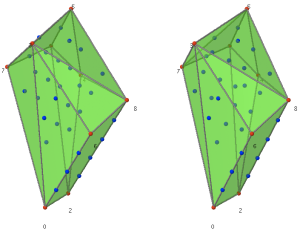
\includegraphics[width=8em]{polytope.png}

Seq\"u\`encies enteres: \texttt{sloane\_find({\it list})}, \texttt{sloane.}$\langle$tab$\rangle$  

Particions:
\texttt{P=Partitions({\it n})}\quad \texttt{P.count()}

Combinacions: \texttt{C=Combinations({\it llista})}\quad\texttt{C.list()}

Producte Cartesi\`a: \texttt{CartesianProduct(P,C)}

Taula: \texttt{Tableau([[1,2,3],[4,5]])}

Paraules: \texttt{W=Words("abc"); W("aabca")}

Posets: \texttt{Poset([[1,2],[4],[3],[4],[]])}

Root systems: \texttt{RootSystem(["A",3])}

Crystals: \texttt{CrystalOfTableaux(["A",3], shape=[3,2])}

Lattice Polytopes: \verb|A=random_matrix(ZZ,3,6,x=7)|

\verb|L=LatticePolytope(A)    L.npoints()   L.plot3d()|

%*********************************************
\hr\textbf{\`Algebra de matrius}

$\begin{pmatrix}1\\2\end{pmatrix}=$ \verb|vector([1,2])|

$\begin{pmatrix}1&2\\3&4\end{pmatrix}=$ \verb|matrix(QQ,[[1,2],[3,4]], sparse=False)|

$\begin{pmatrix}1&2&3\\4&5&6\end{pmatrix}=$ \verb|matrix(QQ,2,3,[1,2,3, 4,5,6])|

$\left|\begin{matrix}1&2\\3&4\end{matrix}\right|=$
\verb|det(matrix(QQ,[[1,2],[3,4]]))|

$Av=$ \verb|A*v| \quad $A^{-1}=$ \verb|A^-1| \quad $A^t=$ \verb|A.transpose()|

Resol $Ax=v$: \verb| A\v  | o \verb| A.solve_right(v)|

Resol $xA=v$: \verb| A.solve_left(v)|

Forma redu\"{\i}da escalonada: \verb| A.echelon_form()|

Rang i dimensi\'o del nucli: \verb|A.rank()    A.nullity()|

Forma de Hessenberg: \verb|A.hessenberg_form()|

Polinomi caracter\'{\i}stic: \verb|A.charpoly()|

Valors propis: \verb|A.eigenvalues()| 

Vectors propis: \verb|A.eigenvectors_right()| (tamb\'e left)

Gram-Schmidt: \verb|A.gram_schmidt()|

Visualitza: \verb|A.plot()|

Reducci\'o: LLL \verb|matrix(ZZ,...).LLL()|

Forma Hermite: \verb|matrix(ZZ,...).hermite_form()|

%*********************************************
\hr\textbf{\`Algebra lineal}

\includegraphics[width=12em,height=6em]{linalg}

Espais de vectors $K^n = $ \verb| K^n | ex. \verb| QQ^3   RR^2   CC^4|

Subespai: \verb|span(vectors, |{\it field}\verb| )| 

Ex., \verb|span([[1,2,3], [2,3,5]], QQ)|

Kernel: \verb|A.right_kernel()| (tamb\'e left)

Suma i intersecci\'o: \verb|V + W | i \verb| V.intersection(W)|

Base: \verb|V.basis()|

Matriu de la base: \verb|V.basis_matrix()|

Restringeix la matriu al subespai: \verb|A.restrict(V)|

Vector en termes de base: \texttt{V.coordinates({\it vector})}

%*********************************************
\hr\textbf{Matem\`atica num\`erica}

Paquets: \verb|import numpy, scipy, cvxopt|

Minimitzaci\'o: \verb|var("x y z")|

\verb|   minimize(x^2+x*y^3+(1-z)^2-1, [1,1,1])|

Ajustament: \verb|var("a b c")|

\verb| dadesx=range(100)|

\verb| dadesy=[1.2*sin(.5*i+.1*random()) for i in dadesx]|

\verb| model(x)=model(x)=a+b*sin(x+c) |

\verb| find_fit(zip(dadesx,dadesy),model) |


%*********************************************
\hr\textbf{Teoria de nombres}

Primers: \verb|prime_range(n,m)|, \verb|is_prime|, \verb|next_prime|

Factor: \verb|factor(n)|, \verb|qsieve(n)|, \verb|ecm.factor(n)|

S\'{\i}mbol de Kronecker: $\left(\frac{a}{b}\right) = $ \texttt{kronecker\_symbol({\it a},{\it b})}

Fraccions continues: \verb|continued_fraction(x)|

Nombres de Bernoulli: \texttt{bernoulli(n)}, \texttt{bernoulli\_mod\_p(p)}

Corbes el$\cdot$l\'{\i}ptiques: \verb|EllipticCurve([|$a_1,a_2,a_3,a_4,a_6$\verb|])|

Car\`acters de Dirichlet : \texttt{DirichletGroup({\it N})}

%Congruence subgroups: \texttt{Gamma0({\it N})}, \texttt{Gamma1({\it N})}, \texttt{GammaH}

Formes modulars: \texttt{ModularForms({\it nivell}, {\it pes})}

S\'{\i}mbols modulars: \texttt{ModularSymbols({\it nivell}, {\it pes}, {\it sign})}

M\`oduls de Brandt: \texttt{BrandtModule({\it nivell}, {\it pes})}

Varietats abelianes modulars: \texttt{J0({\it N})}, \texttt{J1({\it N})}

%*********************************************
\hr\textbf{Teoria de grups}

\texttt{G = PermutationGroup([[(1,2,3),(4,5)],[(3,4)]])}

\texttt{SymmetricGroup({\it n})}, \texttt{AlternatingGroup({\it n})} 

Abelian groups: \texttt{AbelianGroup([3,15])}

Grups de matrius: \texttt{GL, SL, Sp, SU, GU, SO, GO}

Funcions: \texttt{G.sylow\_subgroup(p)}, \texttt{G.character\_table()}, 

\texttt{G.normal\_subgroups()}, \texttt{G.cayley\_graph()}


%*********************************************
\hr\textbf{Anells no commutatius}

Quaternions: \texttt{Q.<i,j,k> = QuaternionAlgebra(a,b)}

\`Algebres Lliures: \texttt{R.<a,b,c> = FreeAlgebra(QQ, 3)}

%Steenrod algebra: \texttt{SteenrodAlgebra({\it prime})}

%*********************************************
\hr\textbf{M\`oduls de Python}

\verb|import| \emph{nom\_del\_m\`odul}

\verb|module_name.|$\langle$tab$\rangle$ i \verb|help(module_name)|

%\verb|sage.|\emph{module\_name}\verb|.all.|$\langle$tab$\rangle$ shows exported commands

%\mbox{Std packages: Maxima GP/PARI GAP Singular R Shell ...}

%Opt packages: Biopython Gnuplot Kash ...

%\%\emph{package\_name} then use package command syntax

%*********************************************
\hr\textbf{Perfils i debugging}

\verb|time| \emph{commanda}: \quad  mostra la informaci\'o temporal

\verb|timeit("command")|: mostra el temps amb m\'es precisi\'o

\verb|t = cputime(); cputime(t)|: temps transcurregut de CPU

\verb|t = walltime(); walltime(t)|: temps transcurregut de wall

\verb|%pdb|: engega el debugger interactiu (nom\'es l\'{\i}nia de comandes)

\verb|%prun command|: comanda de perfil (nom\'es l\'{\i}nia de comandes)

\end{multicols*}

\end{document}
